\let\negmedspace\undefined
\let\negthickspace\undefined
\documentclass[journal]{IEEEtran}
\usepackage[a5paper, margin=10mm, onecolumn]{geometry}
%\usepackage{lmodern} % Ensure lmodern is loaded for pdflatex
\usepackage{tfrupee} % Include tfrupee package

\setlength{\headheight}{1cm} % Set the height of the header box
\setlength{\headsep}{0mm}     % Set the distance between the header box and the top of the text

\usepackage{gvv-book}
\usepackage{gvv}
\usepackage{cite}
\usepackage{amsmath,amssymb,amsfonts,amsthm}
\usepackage{algorithmic}
\usepackage{graphicx}
\usepackage{textcomp}
\usepackage{xcolor}
\usepackage{txfonts}
\usepackage{listings}
\usepackage{enumitem}
\usepackage{mathtools}
\usepackage{gensymb}
\usepackage{comment}
\usepackage[breaklinks=true]{hyperref}
\usepackage{tkz-euclide} 
\usepackage{listings}
\def\inputGnumericTable{}                                 
\usepackage[latin1]{inputenc}                                
\usepackage{color}                                            
\usepackage{array}                                            
\usepackage{longtable}                                       
\usepackage{calc}                                             
\usepackage{multirow}                                         
\usepackage{hhline}                                           
\usepackage{ifthen}                                           
\usepackage{lscape}
\begin{document}

\bibliographystyle{IEEEtran}
\vspace{3cm}

\title{2.6.30}
\author{AI25BTECH11019 - MENAVATH SAI SANJANA}
% \maketitle
% \newpage
% \bigskip
{\let\newpage\relax\maketitle}

\renewcommand{\thefigure}{\theenumi}
\renewcommand{\thetable}{\theenumi}
\setlength{\intextsep}{10pt} % Space between text and floats


\numberwithin{equation}{enumi}
\numberwithin{figure}{enumi}
\renewcommand{\thetable}{\theenumi}

\textbf{Question}:\\
If the area of a triangle is $35$ square units with vertices $(2,6), (5,-4)$ and $(k,4)$, then find $k$.  
\\
\bigskip
\textbf{Solution: }
Let  
$
\overrightarrow{A} = \myvec{2 \\ 6}, \quad 
\overrightarrow{B} = \myvec{5 \\ -4}, \quad 
\overrightarrow{C} = \myvec{k \\ 4}
$

Vectors:  
$
\overrightarrow{B}-\overrightarrow{A} = \myvec{5-2 \\ -4-6} = \myvec{3 \\ -10}, \qquad 
\overrightarrow{C}-\overrightarrow{A} = \myvec{k-2 \\ 4-6} = \myvec{k-2 \\ -2}
$

The area of the triangle is  
$
\text{Area} = \frac{1}{2} \left| (\overrightarrow{B}-\overrightarrow{A}) \times (\overrightarrow{C}-\overrightarrow{A}) \right|
$

$
35 = \frac{1}{2} \left| 
\myvec{3 \\ -10} \times \myvec{k-2 \\ -2} 
\right|
$

So,  
\begin{align*}
35 &= \frac{1}{2}\left| 3(-2) - (-10)(k-2) \right| \\
&= \frac{1}{2}\left| -6 + 10k -20 \right| \\
&= \frac{1}{2}\left| 10k - 26 \right|
\end{align*}

Thus,
$
|10k - 26| = 70
$

\begin{align*}
10k - 26 &= 70  &\Rightarrow \quad k = \frac{48}{5} \\
10k - 26 &= -70 &\Rightarrow \quad k = -\frac{22}{5}
\end{align*}

Therefore,  
$
k = \frac{48}{5} \quad \text{or} \quad k = -\frac{22}{5}
$

\begin{figure}[ht!]
    \centering
    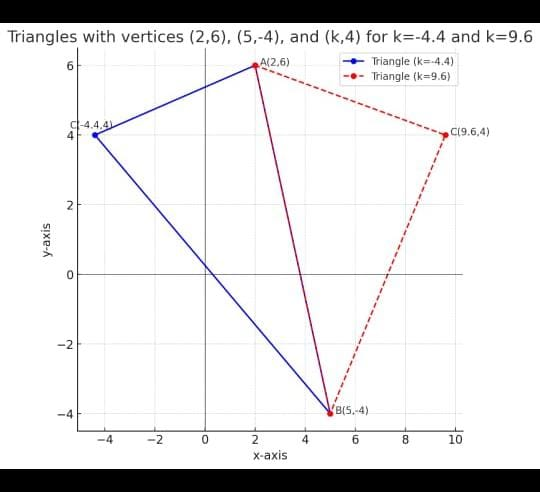
\includegraphics[width=0.8\textwidth]{figs/matgeo-2.6.30.jpeg}
    \caption{}
    \label{fig:1.2.27.jpg}
\end{figure}

\end{document}

